The system recognizes two kind of gestures (see also figure
\ref{fig:gesturesToRecognize}):
\begin{itemize}
  \item A circle that starts from the bottom and runs clockwise
  \item A circle that starts from the bottom and runs counter-clockwise
\end{itemize}
The first gesture is used to mark an item as ``added to cart'' while the second
one serves to switch through the items on the shopping list.

\begin{figure}[h]
\captionsetup{justification=centering}
\begin{subfigure}{0.475\textwidth}
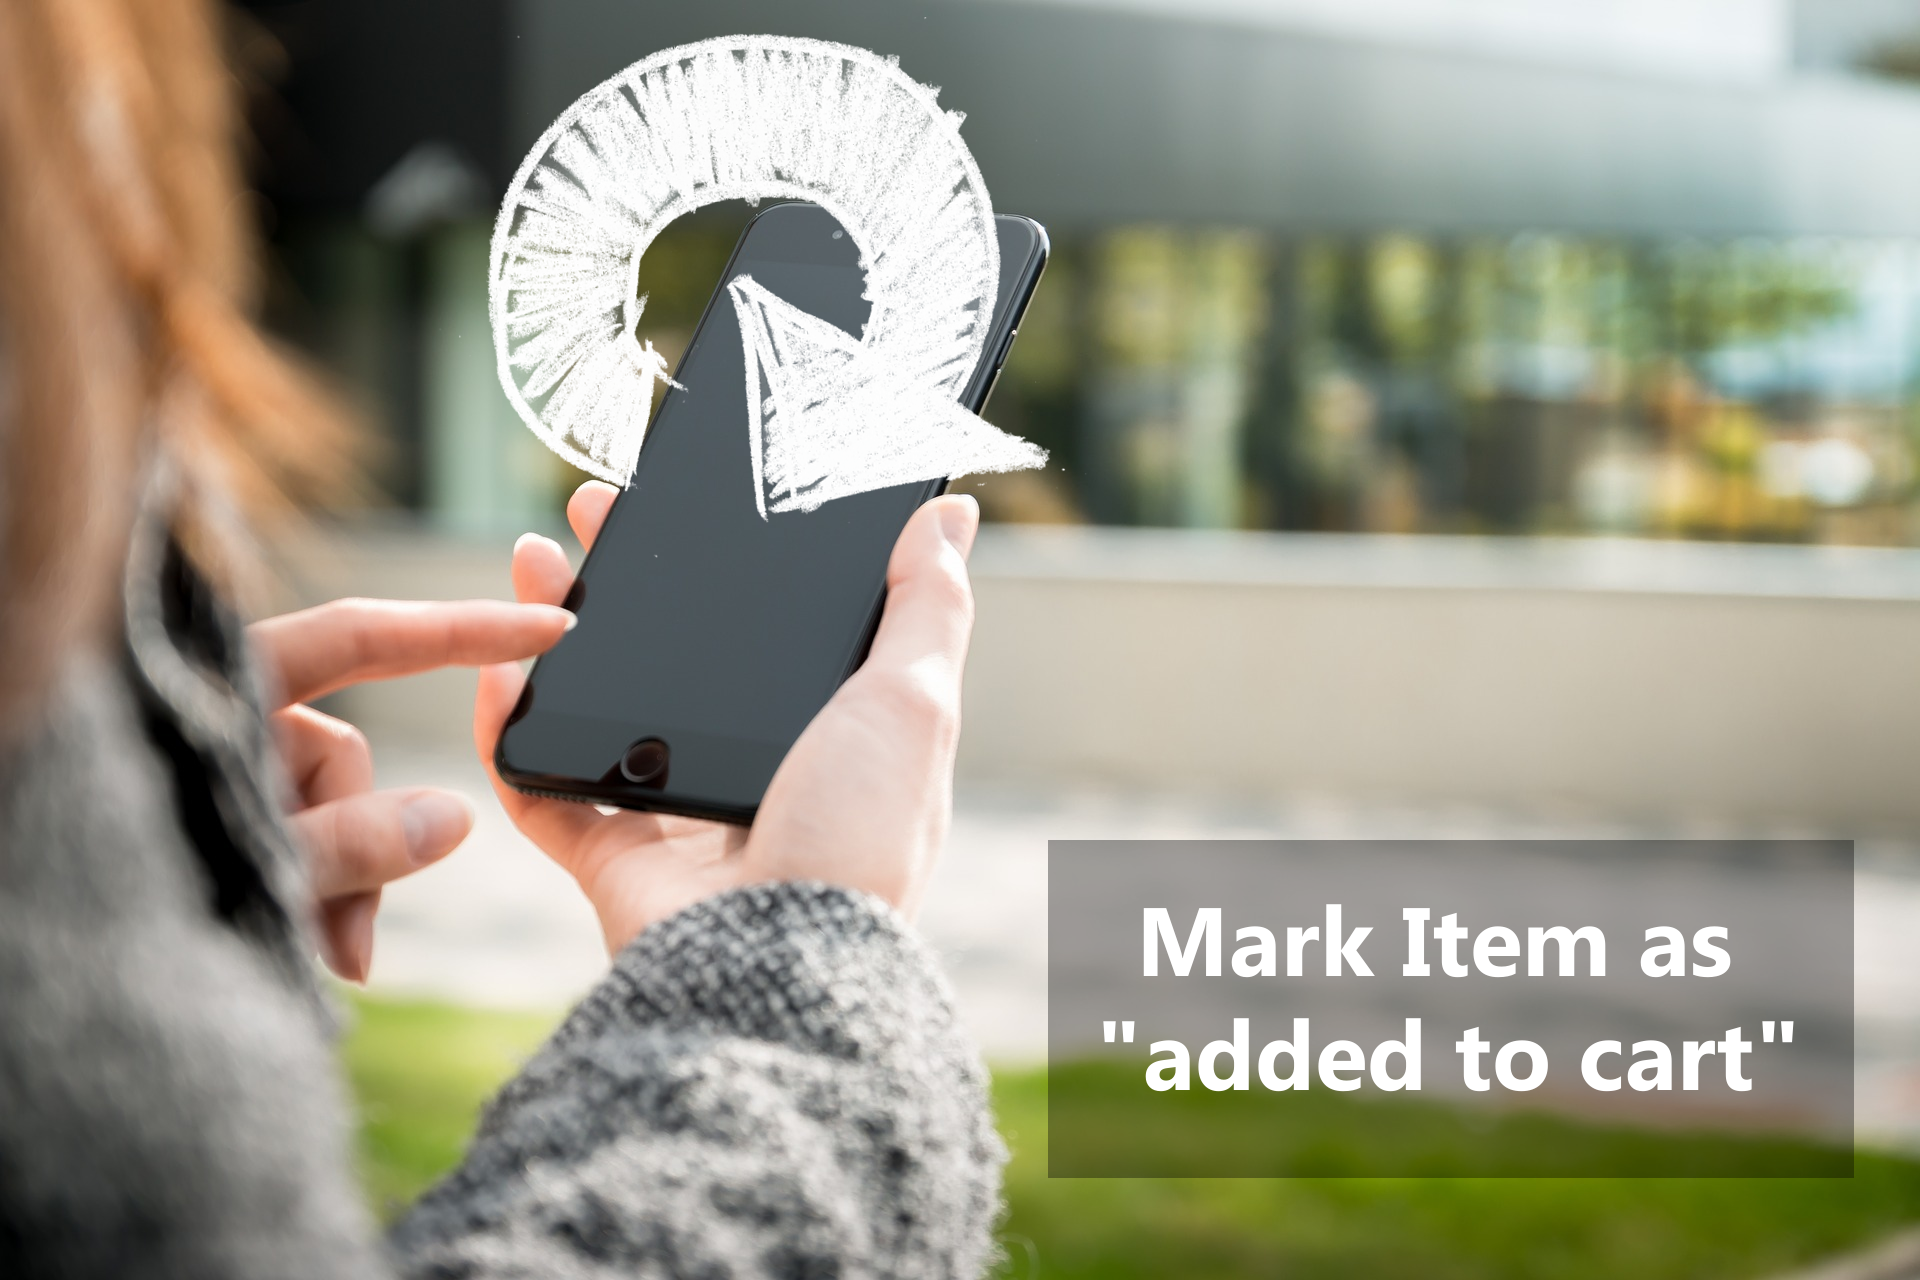
\includegraphics[width=\textwidth]{res/gestures/addToCart.png}
\caption{Add Item to Cart}
\label{fig:gestureAdd}
\end{subfigure} \hspace{0.05\textwidth}
\begin{subfigure}{0.475\textwidth}
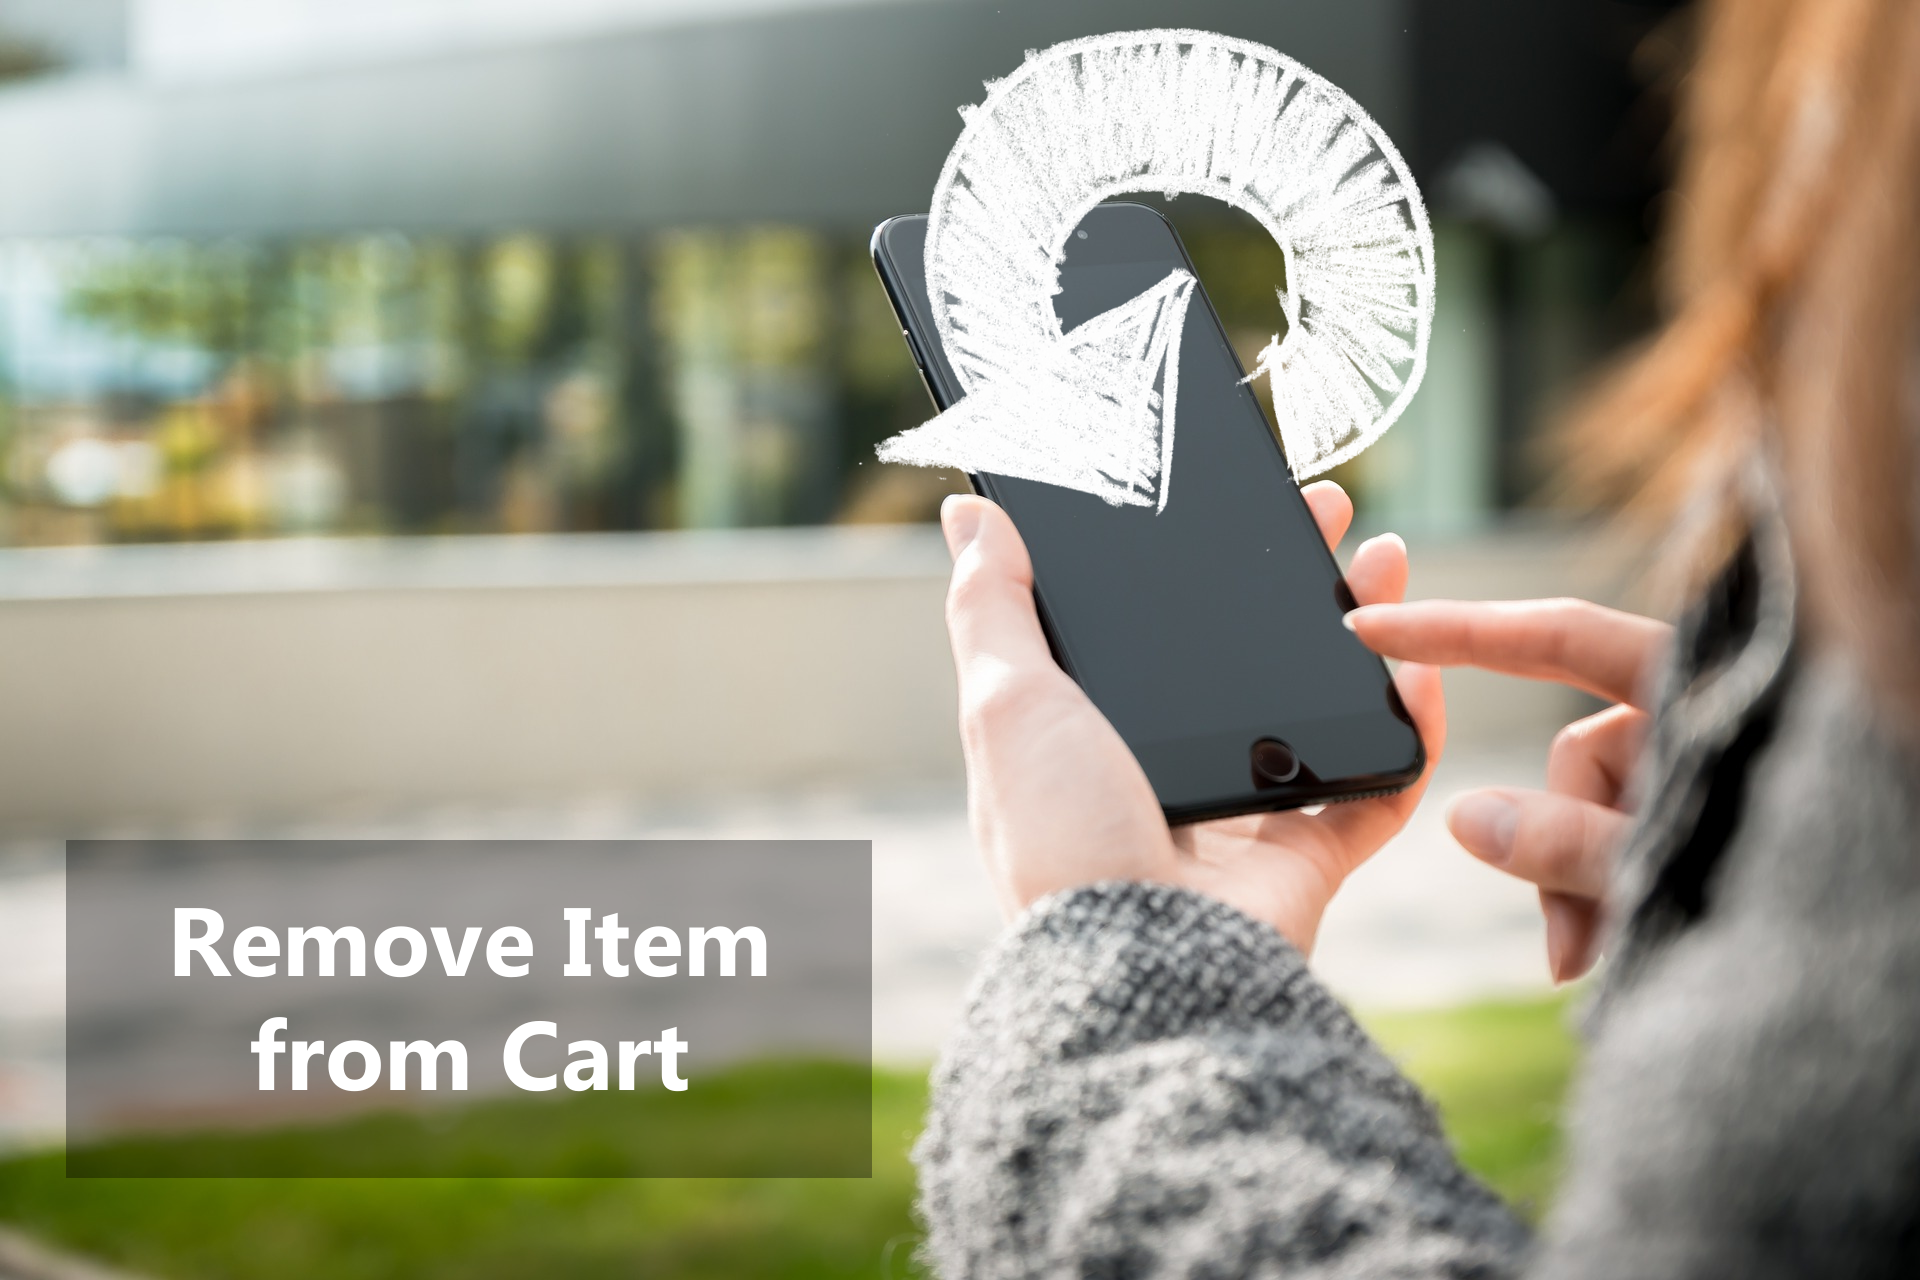
\includegraphics[width=\textwidth]{res/gestures/removeFromCart.png}
\caption{Switch Item}
\label{fig:gestureRemove}
\end{subfigure}
\caption{Gestures to Recognize}
\label{fig:gesturesToRecognize}
\end{figure}

\subsection{Data Analysis and Data Acquisition}

The initial step to achieve gesture recognition via the accelerometer of the
smartphone is to collect data. For this purpose, the Android application
``Accelerometer Analyzer'', which is accessible through the Google Play Store, 
is used to record
acceleration sensor data while performing different gestures.

The diagram \ref{fig:analyzerValues} shows the acceleration distribution across
the smartphone's acceleration axes.

\begin{figure}
\centering
\captionsetup{justification=centering}
\begin{subfigure}{0.45\textwidth}
\begin{tikzpicture}
\begin{axis}[
  id=Measured accelerations,
			width=\textwidth,height=0.25\textheight,
			%title={Measured Accelerations},
    		grid =both,
    		minor x tick num = 1,
    		minor y tick num = 1,
			xlabel={Measurement Point},
			ylabel={Acceleration Values [$\frac{m}{s^2}$]}, ymin=-15, xmin=0,
			xmax=450, legend style={ at={(0,0)}, anchor=south west}] 
\addplot [mark=none, blue, thick] 
		plot table [x=Point, y=x]{res/gestures/kreis_flach_1.csv};
\addlegendentry{$a_x$}
\addplot [mark=none, magenta, thick] 
		plot table [x=Point, y=y]{res/gestures/kreis_flach_1.csv};
\addlegendentry{$a_y$}
\addplot [mark=none, ForestGreen, thick] 
		plot table [x=Point, y=z]{res/gestures/kreis_flach_1.csv};
\addlegendentry{$a_z$}
\end{axis}
\end{tikzpicture}
\caption{planar}
\label{fig:measurementPlanar}
\end{subfigure}
\hspace{0.05\textwidth}
\begin{subfigure}{0.45\textwidth}
\begin{tikzpicture}
\begin{axis}[
  id=Measured accelerations,
			width=\textwidth,height=0.25\textheight,
			%title={Measured Accelerations},
    		grid =both,
    		minor x tick num = 1,
    		minor y tick num = 1,
			xlabel={Measurement Point},
			ylabel={Acceleration Values [$\frac{m}{s^2}$]}, ymin=-15, xmin=0,
			xmax=450, legend style={ at={(0,0)}, anchor=south west}] 
\addplot [mark=none, blue, thick] 
		plot table [x=Point, y=x]{res/gestures/kreis_hochkant.csv};
\addlegendentry{$a_x$}
\addplot [mark=none, magenta, thick] 
		plot table [x=Point, y=y]{res/gestures/kreis_hochkant.csv};
\addlegendentry{$a_y$}
\addplot [mark=none, ForestGreen, thick] 
		plot table [x=Point, y=z]{res/gestures/kreis_hochkant.csv};
\addlegendentry{$a_z$}
\end{axis}
\end{tikzpicture}
\caption{upright}
\label{fig:measurementUpright}
\end{subfigure}
\caption{Retrieved Values for $a_x$, $a_y$ and $a_z$ depending on the Phone's
Orientation}
\label{fig:analyzerValues}
\end{figure}

%TODO: Which gesture is made?
Conducting several measurements, it becomes clear that the acceleration
distribution depends on the orientation of the smartphone. A formula is required
to calculate the smartphone�s acceleration in the direction of x and z
independent its rotation (see chapter \ref{sect:mathBasics}). The values that
are measured if these formulas are applied are depicted in figure
\ref{fig:finalAcc}. Using this measurement, it is possible to define milestone
points to identify a gesture as a circle. 
 
\begin{figure}
\centering
\captionsetup{justification=centering}
\begin{tikzpicture}
\begin{axis}[
  id=Measured accelerations,
			width=0.9\textwidth,height=0.3\textheight,
			%title={Measured Accelerations},
    		grid =both,
    		minor x tick num = 1,
    		minor y tick num = 1,
			xlabel={Measurement Point},
			ylabel={Acceleration Values [$\frac{m}{s^2}$]}, ymin=-15, xmin=0,
			xmax=250, legend style={ at={(0,1)}, anchor=north west}]
\addplot [mark=none, blue, thick] 
		plot table [x=Point, y=a_{x}]{res/gestures/finalExcel.csv};
\addlegendentry{$a_x$}
\addplot [mark=none, ForestGreen, thick] 
		plot table [x=Point, y=a_{z}]{res/gestures/finalExcel.csv};
\addlegendentry{$a_z$}
\end{axis}
\end{tikzpicture}
\caption{Calculated Values $a_x$ and $a_z$ for two Circles}
\label{fig:finalAcc}
\end{figure}

\subsection{Acceleration milestones}

The tables \ref{tab:milestonesCcw} and \ref{tab:milestonesCw} show the defined
acceleration values which have to be reached to recognize a gesture as a circle
in the clockwise/counterclowckwise direction.

In each state the calculated acceleration values in the direction of x or z
respectively have to reach the predefined values within a specified time slot
(0,3s) to get to the next state. Besides that, each state defines a reset value
which resets the current circle recognition. This is necessary to prevent false
positives (e.g. recognizing a circle while shaking the smartphone fast). The
meaning of the presented states is depicted in figure \ref{fig:circleStates}.


\begin{minipage}{0.45\textwidth}
\footnotesize
\begin{tabular}{c|c|c|c}
State & $a_x$ & $a_z$ & Reset Cond. \\
\hline
1 & $< -3$ & $> 3$ & $-$\\
2 & $> 5$ & $> 3$ & $a_z < -5$ \\
3 & $> 5$ & $< -3$ & $a_x < -5$ \\
4 & $< -5$ & $< -3$ & $a_z > 10$ \\
5 & $< -5$ & $> 5$ & $a_x > 5$  
\end{tabular}
\captionof{table}{Milestones: Circle clockwise}
\label{tab:milestonesCw}
\end{minipage}\hspace{0.1\textwidth}
\begin{minipage}{0.45\textwidth}
\footnotesize
\begin{tabular}{c|c|c|c}
State & $a_x$ & $a_z$ & Reset Cond. \\
\hline
1 & $< 3$ & $> 3$ & $-$\\
2 & $< -5$ & $> 3$ & $a_z < -5$ \\
3 & $> 5$ & $< -3$ & $a_x > 5$ \\
4 & $> 5$ & $< -3$ & $a_z > 10$ \\
5 & $> 5$ & $> 5$ & $a_x > -5$  
\end{tabular}
\captionof{table}{Milestones: Circle counter-clockwise}
\label{tab:milestonesCcw}
\end{minipage}

\begin{figure}
\centering
\captionsetup{justification=centering}
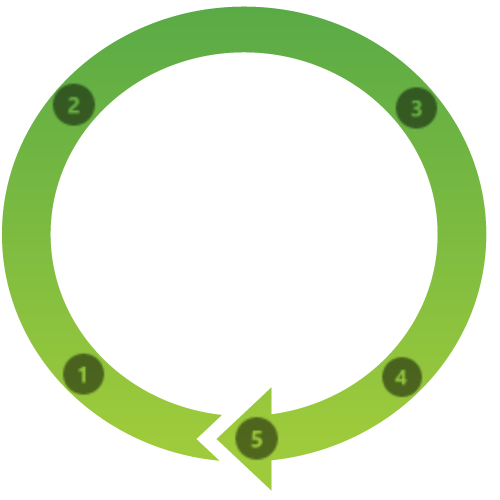
\includegraphics[width=0.4\textwidth]{res/gestures/circleMilestones.png}
\caption{States of the Circle-Recognition}
\label{fig:circleStates}
\end{figure}